\chapter{Classifying Tables Describing Comparisons}
\label{table_classification}
Scientific Research contains a lot of information presented in a tabular structure. These tables hold a lot of relevant information pertaining individual research papers. Since the recent growth of papers on Machine Learning paper and  Neural networks, lots of papers tend to make comparisons with some baselines and other research. Researchers tend to spend a lot of valuable time finding the citations and the table of results from those citations. Sci-Genie via the use of Citation Graph and the Machine Learning models helps filter table describing comparisons at the time of reading research. 

This chapter will cover the problem of classifying tables which describe as comparison of entities and propose approaches to tackle the problem of table type classification. 

\section{Problem Formulation}

The structure of the tables in scientific research can fluctuate based on the information presented by the tables. The tables may also contain information whose context cannot be exactly inferred without the caption underneath the table. Tables occurring in scientific research can also be segregated into well-defined types such as the ones described in Chapter \ref{relatedwork:table-type}. These tables may also not contain a directly linkable entity from a knowledge base(KB) as entities defined in the research may not be present in the KB. Due to such different intrinsic characteristics, models trained using knowledge bases along with web tables such as the one by \cite{deng2020turl} cannot be directly fit to solve this problem. 

\begin{table}
    \label{table\arabic{tablecounter}}
    \centering
    \begin{tabular}{|l|l|l|}
        \hline
        Symbol & Meaning & Type \\ \hline
        $Y$ & Labels & Discrete : $\{0,1\}$ \\ \hline
        $X_T$ & Cell Embedding & $\mathbb{R}^{T_l \times d}$\\ \hline
        $X_C$ & Caption Embedding & $\mathbb{R}^{C_l \times d}$ \\ \hline
        $E_r$ & Row Embedding & $\mathbb{R}^{T_l \times d}$ \\ \hline
        $E_c$ & Column Embedding & $\mathbb{R}^{T_l \times d}$ \\ \hline
        $T_l$ & Number Of Cells & $\mathbb{N}$ \\ \hline
        $T_r$ & Number Of Rows & $\mathbb{N}$ \\ \hline
        $T_c$ & Number Of Columns & $\mathbb{N}$ \\ \hline
        $C_l$ & Length of Caption & $\mathbb{N}$ \\ \hline
        $T_{cell}$ & Sequnces of Cells & $\mathbb{N}^{T_l}$ \\ \hline
        $f_\theta$ & Neural Network & - \\ \hline
    \end{tabular}
    \caption{\label{tablecounter} Table Of Symbols for Equations}
\end{table}
\refstepcounter{tablecounter}
The problem of classifying a table $T$ as a table describing a comparison can be framed as a binary classification problem. Given a table $T$ and its caption $C$, the classifier $f_\theta(T,C) \rightarrow Y$ predicts a binary label $Y \in \{0,1\}$ to denote weather the table is describing a comparison of entities. 

Based on this formulation, this dissertation analyzes 3 different types of ML models and the representations they use for the table $T$ and caption $C$ for the problem:
\begin{itemize}
    \item Cross Channel Transformers With/Without Pretraining
    \item Finetuning Pretrained Scibert
    \item SVM and Naive Bayes (Baselines)
\end{itemize}

Section \ref{table_classification:models} describes the models developed/trained for the input representations of table $T$ and caption $C$. The data collection and labeling for the machine learning models is described in Section \ref{table_classification:data-coll}. The experiment results for different models is described in Section \ref{table_classification:experiement-result}

\section{Classification Models}
\label{table_classification:models}

\subsection{Cross Channel Transformer}
\begin{figure}[h]
    \centering
    \includegraphics[width=\maxwidth{\textwidth}]{src/images/TabTrans.pdf}
    \caption{Cross Channel Transformer For Table Classification}
    \label{figure\arabic{figurecounter}}
\end{figure}
\refstepcounter{figurecounter}

Based on the models developed by \cite{deng2020turl} and \cite{tsai2019multimodal}, a cross channel Transformer model is adapted to fit the function $f_\theta$. Figure \ref{figure15} shows the outline of the model.

\subsubsection{Input Representation}
Each table $T$ is represented as tuple of $(T_{cell},E_r,E_c)$; where $T_{cell} \in \mathbb{N}^{T_l}$ are the cells of the table represented as a sequence of integer tokens; $E_r$ is the row embedding where any index $E_{r_{i}}$ represents the row of the cell $T_{cell_{i}}$ as an embedding;  $E_c$ is the column embedding where an embedding at any index $E_{c_{i}}$ represents the column of the cell $T_{cell_{i}}$ as an embedding. The caption $C$ is represented as sequence of integer tokens which will be transformed to embeddings by the Transformer Model. The representations for the table $T$ are inspired from the models created by \cite{deng2020turl}. 

The cell sequence tokens $T_{cell}$ and caption $C$ are created using a word-piece tokenizer from the SciBert Model \footnote{https://huggingface.co/allenai/scibert\_scivocab\_uncased}. The tokenizer converts the value of individual cells or the caption into a sequence of integer tokens. These tokens can later be used to create embeddings which are passed to the  transformer model. 

\subsubsection{Model Description}
The table cell sequence $T_{cell}$ and the Caption $C$ are first converted to embeddings $X_T, X_C$ respectively. Post creation of the embeddings,  the caption embedding  $X_C$ is added with the position embedding $P_C$; The cell embeddings $X_T$ are added with $E_r,E_c$. After the additions of the respective embeddings, differentiable CLS tokens are concatenated to $X_T,X_C$.
These embeddings are passed to separate cross channel attention transformer layers \parencite{tsai2019multimodal} after which they are passed to the vanilla transformer encoder attention layers \parencite{vaswani2017attention}. For the table of comparison classification task embeddings at the position of the CLS token are pooled from the sequences and concatenated. Once concatenated, this joint embedding is passed to feed forward layers for classification using Cross Entropy Loss. For the pretaining task, the output from the last vanilla encoder layer will be used for predicting the masked tokens of the input table cells $T_{cell}$ and the caption $C$.


\subsubsection{Pretraining Task}
Based on the insights learned from \cite{hernandez2021scaling} on the effectiveness of pretrained models for downstream tasks, the cross-channel transformer model is pretrained with 70K tables from papers from ArXiv. A masked language modeling pretraining objective is used to train the Transformer model given in Figure \ref{figure15}. The pretraining follows the procedures described by \cite{deng2020turl} where the task is of Mask Language Modeling for the sequence of cells $T_{cell}$ and the caption $C$. The model is tasked to predict the word token where a MASK token is inserted in the sequence.  This objective allows training the model with Large number of tables instead of using classifiers trained on small amounts of data. 

\subsubsection{Model Training}
The cross channel transformer model is first pretrained and then fine-tuned for 40 epochs for the task of table classification with a learning rate of 0.0001 scheduled by a cosine learning rate scheduler. 

\subsection{Finetuning Scibert Transformer Model}
\cite{beltagy2019scibert} created a model which was trained on large full text corpus of scientific research containing 1.14M research papers. As this model has been subjected large amounts of pretraining, it is chosen for fine tuning for the same problem as the model may have encountered data of a similar distribution. 
\subsubsection{Input Representation}
\label{table_classification:models:sb:input_rep}
For the finetuning of SciBert, The Table $T$ and caption $C$ are serialized to strings and one concatenated string is created. An example representation is given below: 
\begin{verbatim}
    CAPTION : Table 1: Feature extraction time (Seconds), 
    number of parameters (Millions), and network size (Megabytes) 
    for each source on Office + Caltech-10 datasets.

    TABLE :                          0         1           2      3
0                     Task  Net size  Parameters   Time
1          Squeezenet [17]        46        1.24   13.3
2             Alexnet [21]       227          61   13.9
3           Googlenet [40]        27           7   15.9
4          Shufflenet [51]       6.3         1.4   17.0
5            Resnet18 [15]        44        11.7   14.8
6               Vgg16 [36]       515         138   33.6
7               Vgg19 [36]       535         144   37.1
8         Mobilenetv2 [35]        13         3.5   21.4
9        Nasnetmobile [55]        20         5.3   39.3
10           Resnet50 [15]        96        25.6   22.7
11          Resnet101 [15]       167        44.6   26.7
12        Densenet201 [16]        77          20   61.8
13        Inceptionv3 [41]        89        23.9   28.2
14            Xception [4]        85        22.9   48.1
15  Inceptionresnetv2 [39]       209        55.9   54.1
16        Nasnetlarge [55]       360        88.9  141.2
\end{verbatim}

\subsubsection{Model Description}
The input representation string is converted to a sequence of integer tokens which are capped to the length of 512 tokens because of SciBert's constraint on maximum sequence length. A class token is added at the start of the sequence and the sequence is passed to the Scibert Model. The class token is pooled from after the final layer and is passed to a feed forward neural network for binary classification using cross entropy loss. 

\subsubsection{Model Training}
The model is trained using the for 6 epochs with a linear learning rate warm up schedule of 20 epochs.

\subsection{Baselines}
SVM models are used as baselines as when \cite{kim2012scientific} conducted a study for table type classification, deep learning was not as popular. Naive Bayes(NB) model are also chosen as an additional baseline for the classification task. 

\subsubsection{Input Representation}
The input representation for the SVM and the NB model are the same as the string described in Section \ref{table_classification:models:sb:input_rep}. The string undergoes tokenisation and a classifier is trained based on TF/IDF values of the input strings. 


\section{Data Collection And Labeling}
\label{table_classification:data-coll}

\begin{figure}[h]
    \centering
    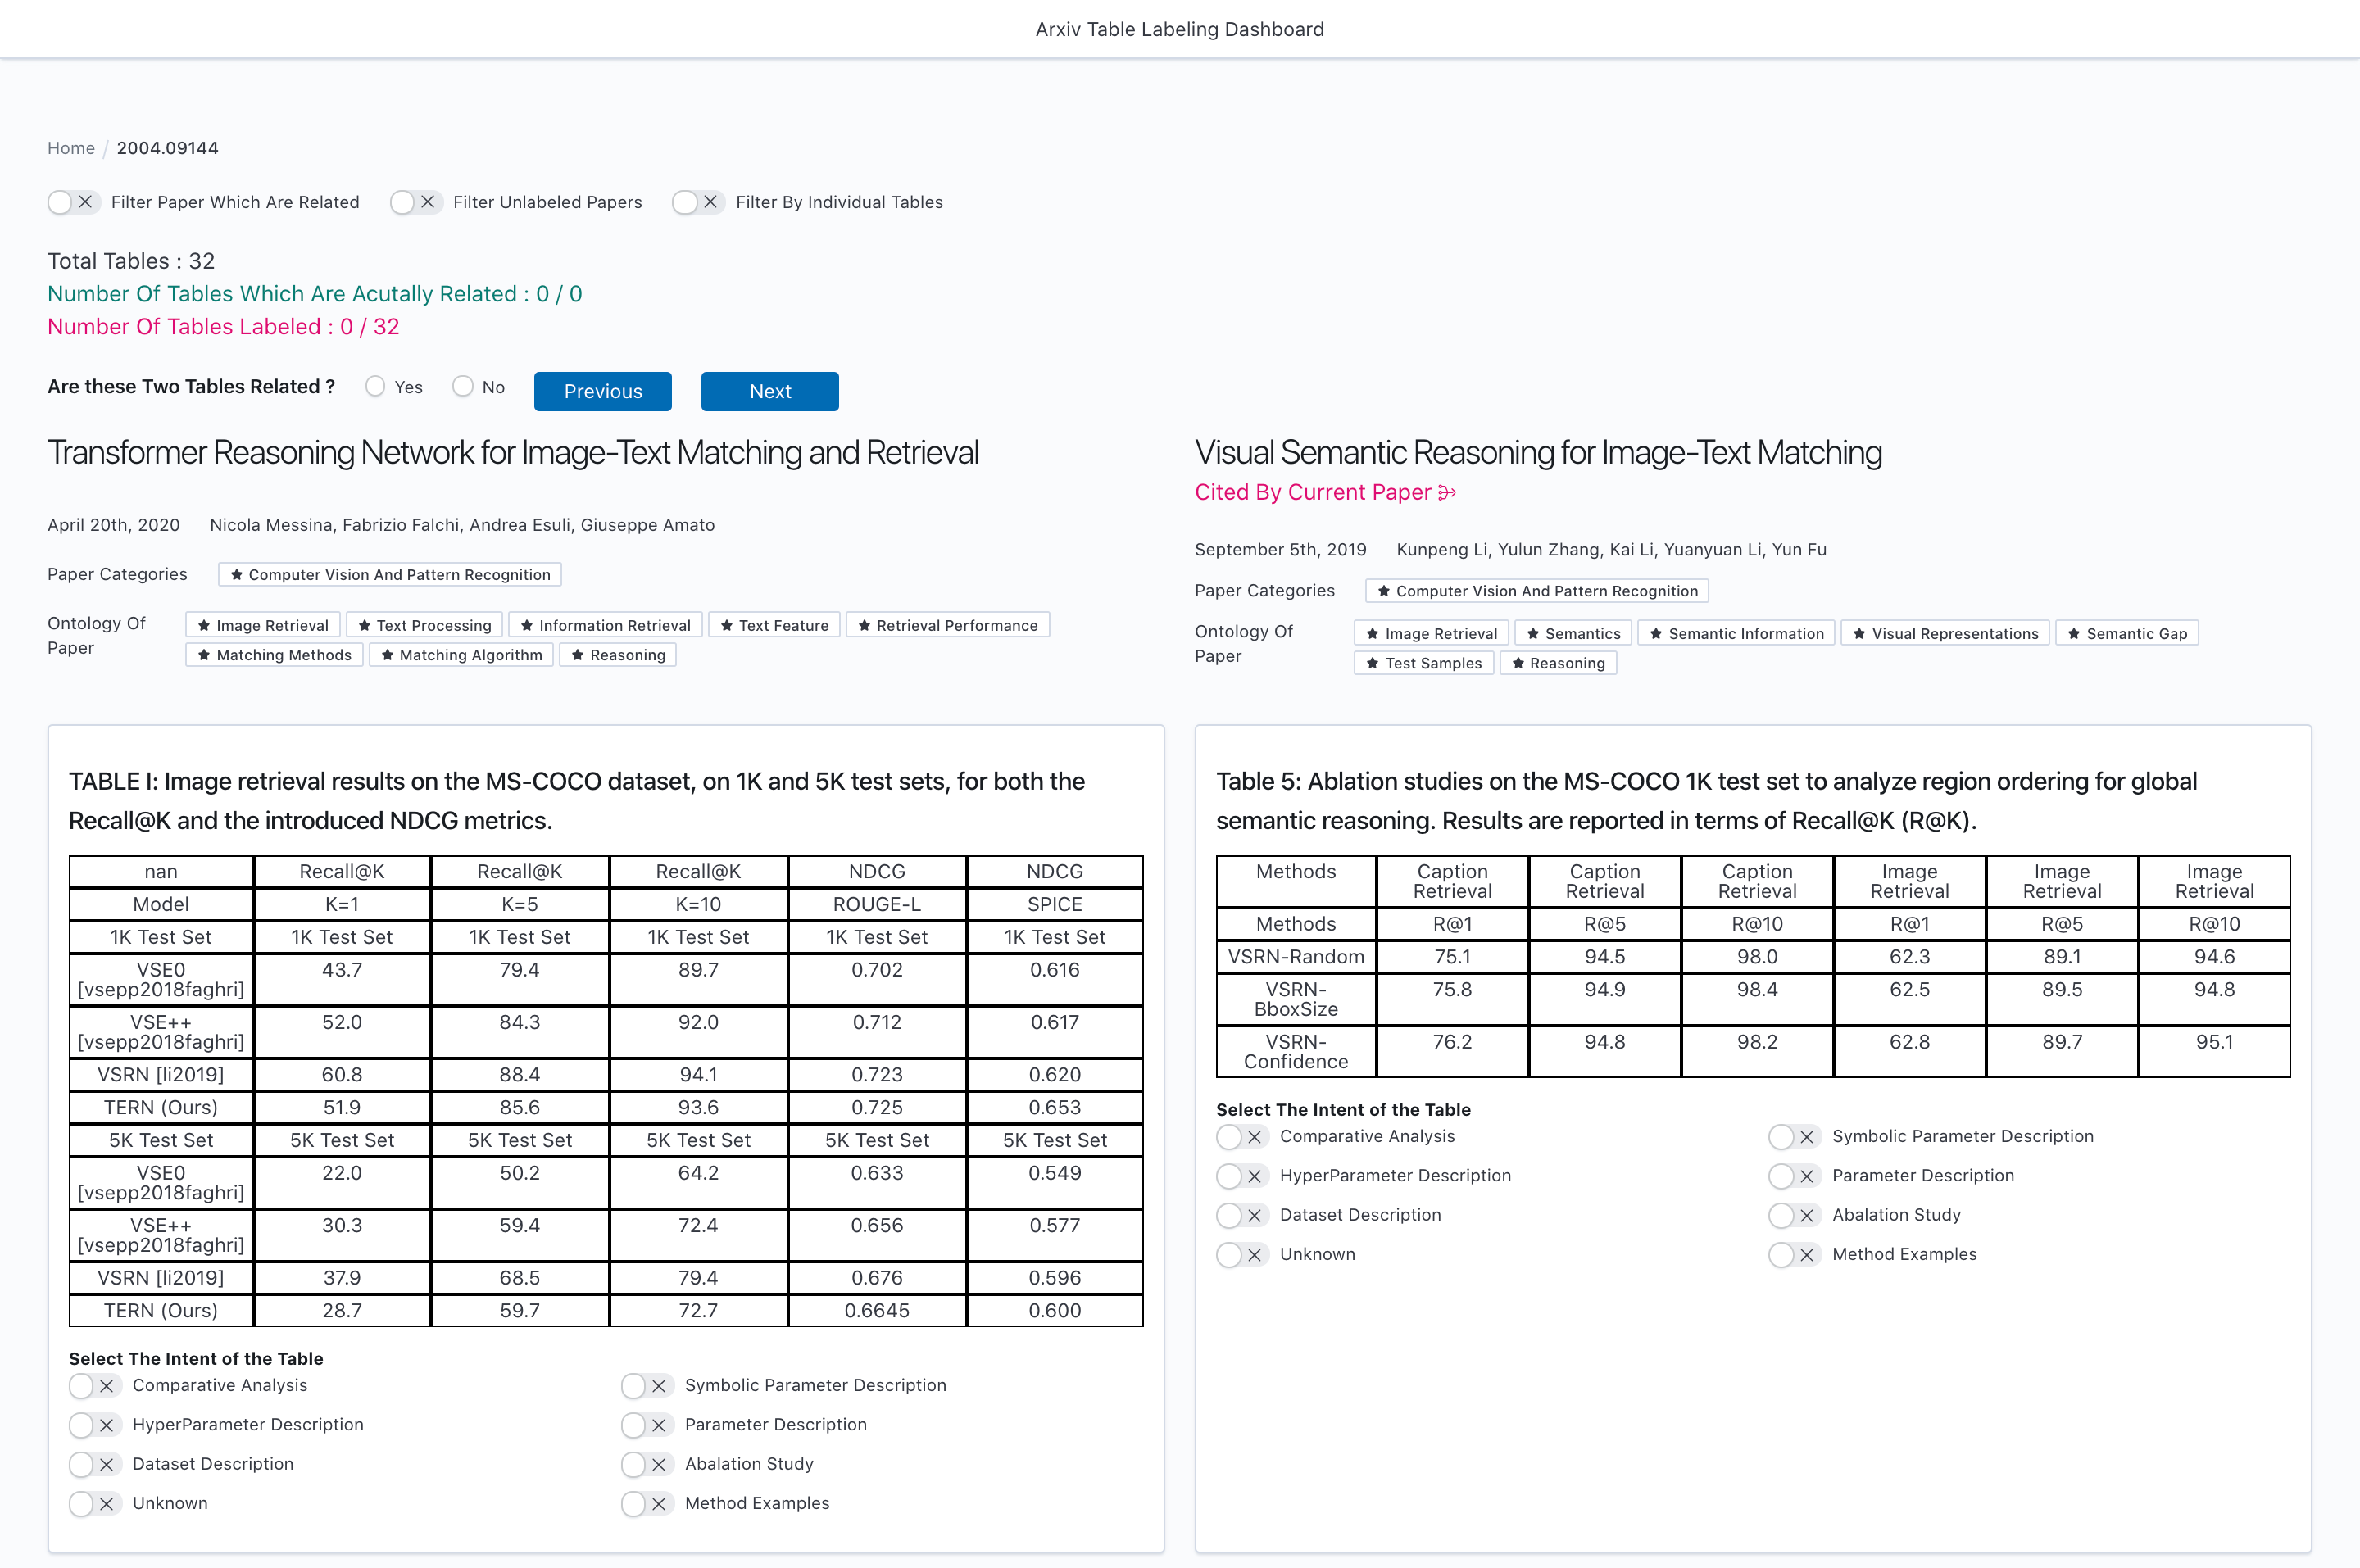
\includegraphics[width=\maxwidth{\textwidth}]{src/images/table-label-interface.png}
    \caption{Table Labeling Interface For Table Relation and Intent Annotation}
    \label{figure\arabic{figurecounter}}
\end{figure}
\refstepcounter{figurecounter}

As Sci-Genie consists of a Data Layer (Chapter \ref{sci-genie-core:data-layer}) that contains the tables from the research papers, A labeling interface(Figure \ref{figure16}) is designed to annotate tables from 240 research papers. 820 tables are annotated out of which 574 tables are describing a comparison and 246 are not. The labeling interface supports labeling types to tables described by \cite{kim2012scientific} and few more based on the observations from current CS research. More details regarding this subject are discussed in Chapter \ref{conclusion:future-scope:type-class}. 

\section{Experiment Results}
\label{table_classification:experiement-result}
\begin{table}[h]
    \label{table\arabic{tablecounter}}
    \centering
    \begin{tabular}{|l|l|l|l|}
    \hline
        \textbf{Model} & \textbf{Accuracy} (\%) & \textbf{F1 Score}  & \textbf{Loss} \\ \hline
        Naive Bayes & 71.6 & 0.825 & - \\ \hline
        SVM  & 78.39 & 0.85477 & - \\ \hline
        Table Cross Channel Transformer Pretained & 85.45 & 0.86 & 0.39 \\ \hline
        Table Cross Channel Transformer From Scratch & 79.23 & 0.79 & 0.53 \\ \hline
        SciBert Finetuned & 92.624 & 0.92 & 0.14 \\ \hline
    \end{tabular}
    \caption{\label{tablecounter} Results of the Experiments For Table Classification Using SOTA Transformer. Average Results from 5 Training runs is reported}
\end{table}
\refstepcounter{tablecounter}
The following are the experiement and thier conditions for ML model training:
\begin{itemize}
    \item Table Cross Channel Transformer : Pretrained with 70K Tables and finetuned on classification task
    \item Table Cross Channel Transformer : Direct trained from scratch on classification task 
    \item SciBert : Finetuned on classification task.
    \item Naive Bayes \& SVM
\end{itemize}
More details on the hyper parameters for the experiments are found in the Appendix \ref{appendix:toc}.
All experiments are conducted using Google Colab Notebooks on NVIDIA P100 GPUs. Table \ref{table5} describes the results of the experiments. The Cross channel model when pretrained generally performs better than the model trained from scratch or even the baseline models. The SciBert out performs all other models. Some inferences can be made based on the study by \cite{hernandez2021scaling}. As SciBert was trained on much bigger corpuses, it's performance is better than the baseline and the developed model. It can be also be inferred from the study by \cite{hernandez2021scaling} that models like Scibert which are bigger and pretrained on more data would generally perform better on downstream tasks. It can also be seen from Table \ref{table5} that pretraining has a direct influence on a better model compared training the model from scratch. As the SciBert model is much larger, the realtime classfication of tables describing comparsions is done using the pretrained cross channel model which is much smaller than the SciBert model.  